\documentclass[letterpaper, 11pt]{article}

\usepackage{tikz, listings, comment}
\usepackage[fleqn]{amsmath}
\usepackage[margin=1in]{geometry}
\usepackage{fancyhdr, hyperref, pdfpages}
\usepackage{xcolor}
\usepackage{float} % Add this to your preamble if not already included

\definecolor{codegreen}{rgb}{0,0.6,0}
\definecolor{codegray}{rgb}{0.5,0.5,0.5}
\definecolor{codepurple}{rgb}{0.58,0,0.82}
\definecolor{backcolour}{rgb}{0.95,0.95,0.92}

% Disable page numbers
\pagestyle{empty}

%Basic Variables (Modify as required per homework)
\def\class{CompEn 462}
\def\homeworkNumber{Final Project}
\def\date{05.07.2025}
\def\professor{Mark Mahon}

% Define a custom style for listings
\lstdefinestyle{mystyle}{
    backgroundcolor=\color{backcolour},   % Set background color for the code block
    commentstyle=\color{codegreen},       % Set color for comments
    keywordstyle=\color{magenta},         % Set color for keywords
    numberstyle=\tiny\color{codegray},    % Set style for line numbers
    stringstyle=\color{codepurple},       % Set color for strings
    basicstyle=\ttfamily\footnotesize,    % Set basic style for the code
    breakatwhitespace=false,              % Do not break lines at whitespace
    breaklines=true,                      % Allow breaking of lines
    captionpos=b,                         % Set caption position to bottom
    keepspaces=true,                      % Keep spaces in text
    %numbers=left,                         % Display line numbers on the left
    numbersep=5pt,                        % Set distance between line numbers and code
    showspaces=false,                     % Do not show spaces
    showstringspaces=false,               % Do not show spaces in strings
    showtabs=false,                       % Do not show tabs
    tabsize=2                             % Set tab size to 2 spaces
}

\lstset{style=mystyle}

%Code to generate new page for problem
\newcounter{problemId}
\stepcounter{problemId}
\def\newproblem{\clearpage\newpage\noindent{Problem~\arabic{problemId}\stepcounter{problemId}}\hfill\par}

%Custom Section Header Command
\newcommand{\secHeader}[1]{\vspace{2mm} \noindent \textbf{#1:}\vspace{-4mm}}

\begin{document}
%Title page
\hfill
\newline
Name: Justin Ngo
\\PSU ID: jvn5439
\\Professor: \professor
\\Class: \class
\\Date: \date
\\Project : Wireless MAC Address Spoofing Detection System Using ESP32

%---------------------ABSTRACT---------------------
\newpage
\secHeader{Abstract}
\vspace{5mm}

The purpose of this project is to use an ESP32 microcontroller to create a device that passively detects wireless connections to an access point and logs the MAC addresses and RSSI of the various
connections that are made. The device operates in two modes: learning and monitoring. When the device detects that there are no known connections in the known\_connections\_file, it will enter
learning mode and begin logging the MAC addresses and corresponding RSSI of the connections that are made for the next 2 minutes and 30 seconds. Assuming that these connections are "normal" connections,
the device will save these MAC addresses and their corresponding RSSI values to the known\_connections\_file and use that as a sort of whitelist of valid MAC addresses. 
After the learning period, the device will enter monitoring mode and try to determine if the MAC address of incoming traffic is a spoofed MAC address or not by comparing the RSSI of any new connections
to the RSSI of other connections that were made recently. 


%---------------------OUTLINE---------------------
\newpage
\secHeader{Outline}
\vspace{5mm}

The main idea behind this project was just to experiment with the ESP32 microcontroller and see if I could get it to detect wireless connections made to the access point in my apartment living room.


\secHeader{Tools and Libraries}
\vspace{5mm}
\begin{enumerate}
    \item Arduino Nano ESP32 Microcontroller: this was the main hardware part used in the project. I selected it primarily because it was easy to get and I have a little experience with using other 
    Arduino microcontrollers.
    \item Arduino IDE: all the code was done in the Arduino IDE. I selected this IDE because I have prior experience with it from another class and remember it being fairly intuitive to use
    \item SPIFFS Library: the SPIFFS library is what allowed the ESP32 to create a JSON file on its onboard flash memory. I found out about it while looking for a way to save the packet information
    to a file for the device to reference later.
    \item Wifi Library: the Wifi library allowed the ESP32 to connect to the same wifi network as my computer. I'm not sure that it was entirely necessary to go through with adding the ESP32 to the 
    network but did so anyway to ensure that it was properly scanning the network for connections.
    \item ESP32 Wifi Library: I used this library to set the ESP32 in promiscuous mode. This library is core to the device's functionality as it's what allows the ESP32 to detect the 
    MAC addresses and RSSI of the connections that are made to the access point.
    \item ArduinoJson Library: I used this to maintain the JSON file which stored the known connections that the device learned during its learning phase.
\end{enumerate}


\newpage
\secHeader{Code Walkthrough}
\vspace{5mm}

\begin{figure}[H] % Use [H] to force the figure to stay here
    \centering
    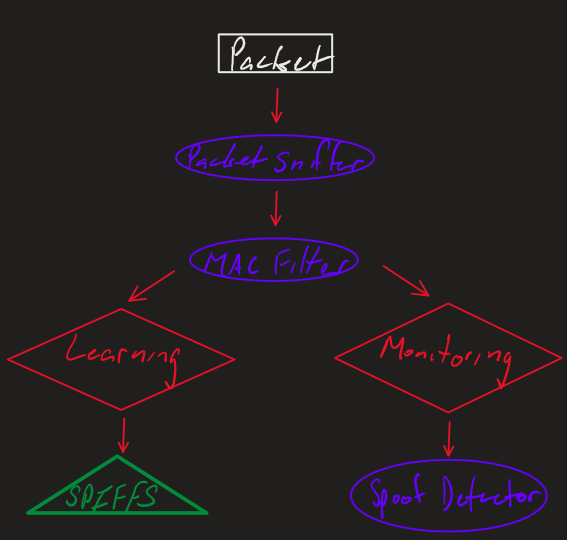
\includegraphics[width=0.8\textwidth]{Diagram.png}
    \caption{System Diagram}
    \label{fig:SystemDiagram}
\end{figure}

The figure above shows a very general overview of how the system works. The ESP32 detects packets in promiscuous mode which are then processed by the Packet Sniffer function. The MAC 
Filter removes packets to or from the other access points on the network and also ignores packets sent to FF:FF:FF:FF:FF:FF, which is the broadcast address to prevent the device from
flooding the storage with unnecessary packets. Depending on what mode the device is currently operating in, the device will either save the packet information to the known\_connections\_file 
or compare the RSSI of the incoming packet to the RSSI of the other recently received packets to try and determine if it's coming from a spoofed MAC address.


\end{document}